\documentclass[twocolumn,a4j]{jsarticle}
\setlength{\topmargin}{-20.4cm}
\setlength{\oddsidemargin}{-10.4mm}
\setlength{\evensidemargin}{-10.4mm}
\setlength{\textwidth}{18cm}
\setlength{\textheight}{26cm}

\usepackage[top=15truemm,bottom=20truemm,left=15truemm,right=15truemm]{geometry}
\usepackage[latin1]{inputenc}
\usepackage{amsmath}
\usepackage{amsfonts}
\usepackage{amssymb}
\usepackage[dvipdfmx]{graphicx}
\usepackage[dvipdfmx]{color}
\usepackage{listings}
\usepackage{listings,jvlisting}
\usepackage{geometry}
\usepackage{framed}
\usepackage{color}
\usepackage[dvipdfmx]{hyperref}
\usepackage{ascmac}
\usepackage{enumerate}
\usepackage{tabularx}
\usepackage{cancel}
\usepackage{scalefnt}

\renewcommand{\figurename}{Fig.}
\renewcommand{\tablename}{Table }

\lstset{
basicstyle={\ttfamily},
identifierstyle={\small},
commentstyle={\smallitshape},
keywordstyle={\small\bfseries},
ndkeywordstyle={\small},
stringstyle={\small\ttfamily},
frame={tb},
breaklines=true,
columns=[l]{fullflexible},
xrightmargin=0zw,
xleftmargin=3zw,
numberstyle={\scriptsize},
stepnumber=1,
numbersep=1zw,
lineskip=-0.5ex
}

\makeatletter
\def\@maketitle
{
\begin{center}
{\LARGE \@title \par}
\end{center}
\begin{flushright}
{\large 報告書 NO.09 - 2\quad\@date\quad\@author}
\end{flushright}
\par\vskip 1.5em
}
\makeatother

\setcounter{tocdepth}{3}

\author{来代 勝胤}
\title{令和3年度 1月 第2週 報告書}
\date{2022/1/13}

\begin{document}
\columnseprule=0.1mm

\maketitle
\section*{報告内容}
\begin{enumerate}[1.]
    \item 進捗状況
    \item 実験データ
    \item 校正装置と供試体のオフセット
    \item テストデータへの補正プログラム適用結果
    \item 次週の予定
\end{enumerate}

\section{進捗状況}
評価実験の結果に軸の回転を考慮した補正値を用いて,正味出力電圧を算出したところ
そのプロットした図(Fig.1)に周期的な振動が見られた.
今週は,その原因と考えられる校正装置と供試体の軸のオフセットを考慮したテストデータを作成し
補正プログラムを適用した出力結果と実験結果の比較を行った.

\section{実験データ}
以前の実験結果について以下のFig.1~Fig.4,その算出値をTable 1に示す.

\begin{itemize}
    \item [$\blacksquare$] \textgt{出力電圧の傾き(補正前)}
\end{itemize}

\begin{figure}[htbp]
    \footnotesize
    \begin{center}
        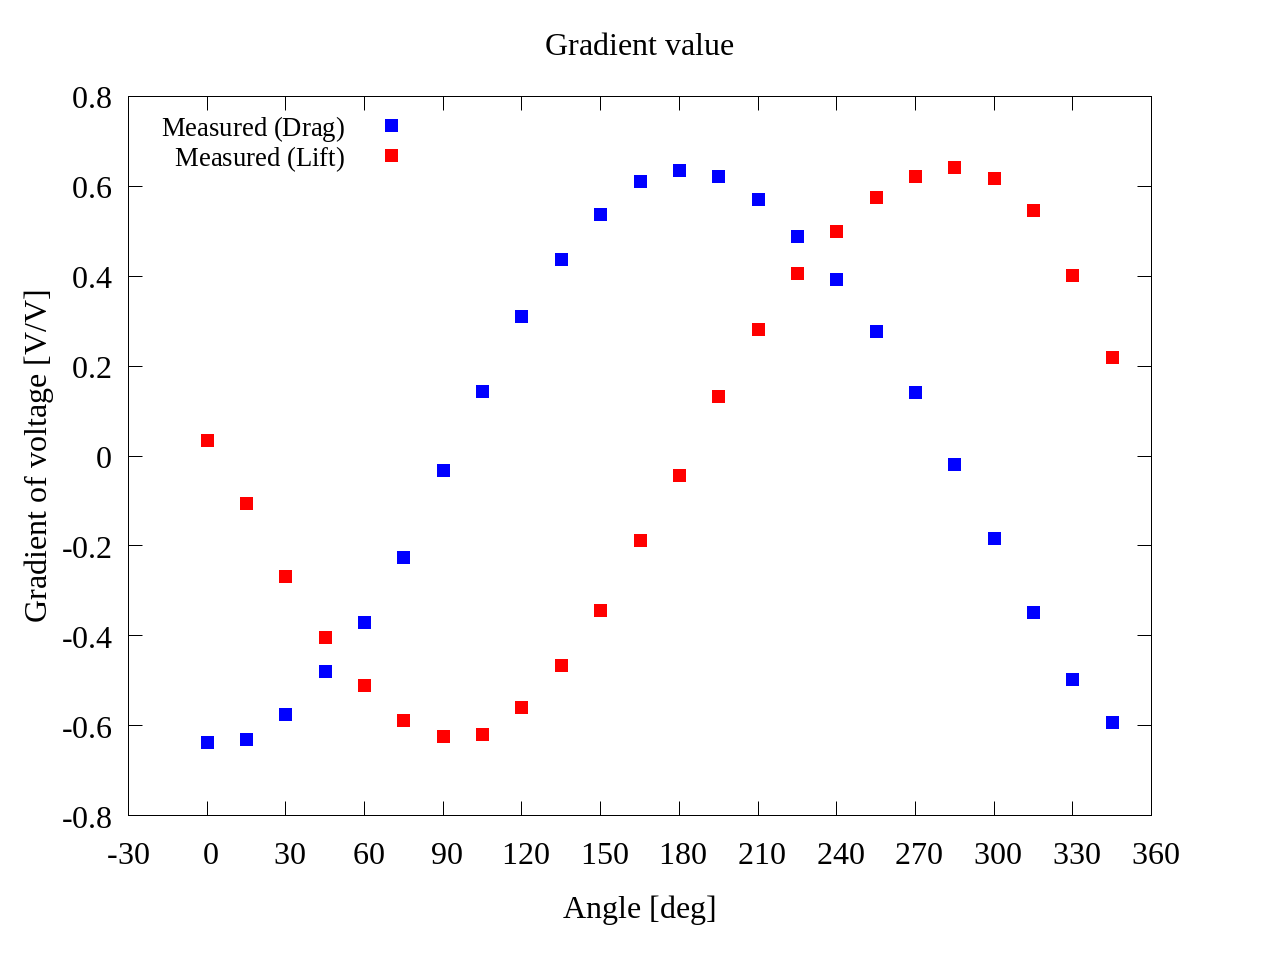
\includegraphics[width=86mm]{../graphes/1-ex/05/05_summary-wave.png}
        \caption{Summary of gradient voltage (Measured)}
    \end{center}
\end{figure}

\newpage

\begin{itemize}
    \item [$\blacksquare$] \textgt{出力電圧の傾き(補正後)}
\end{itemize}

\begin{figure}[htbp]
    \footnotesize
    \begin{center}
        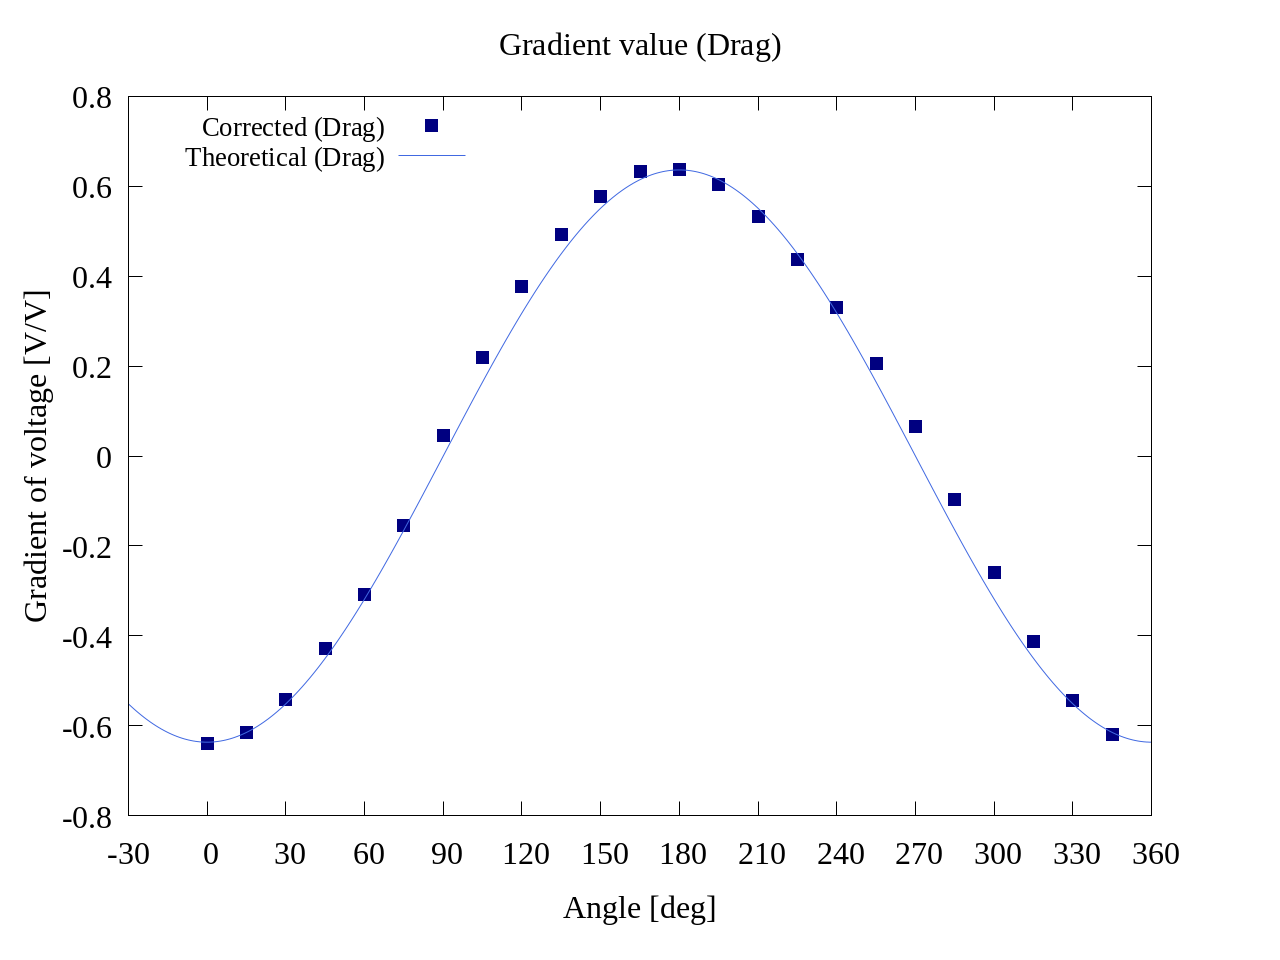
\includegraphics[width=86mm]{../graphes/1-ex/21/21-2_corrected_drag.png}
        \caption{Summary of drag's gradient voltage (corrected)}
        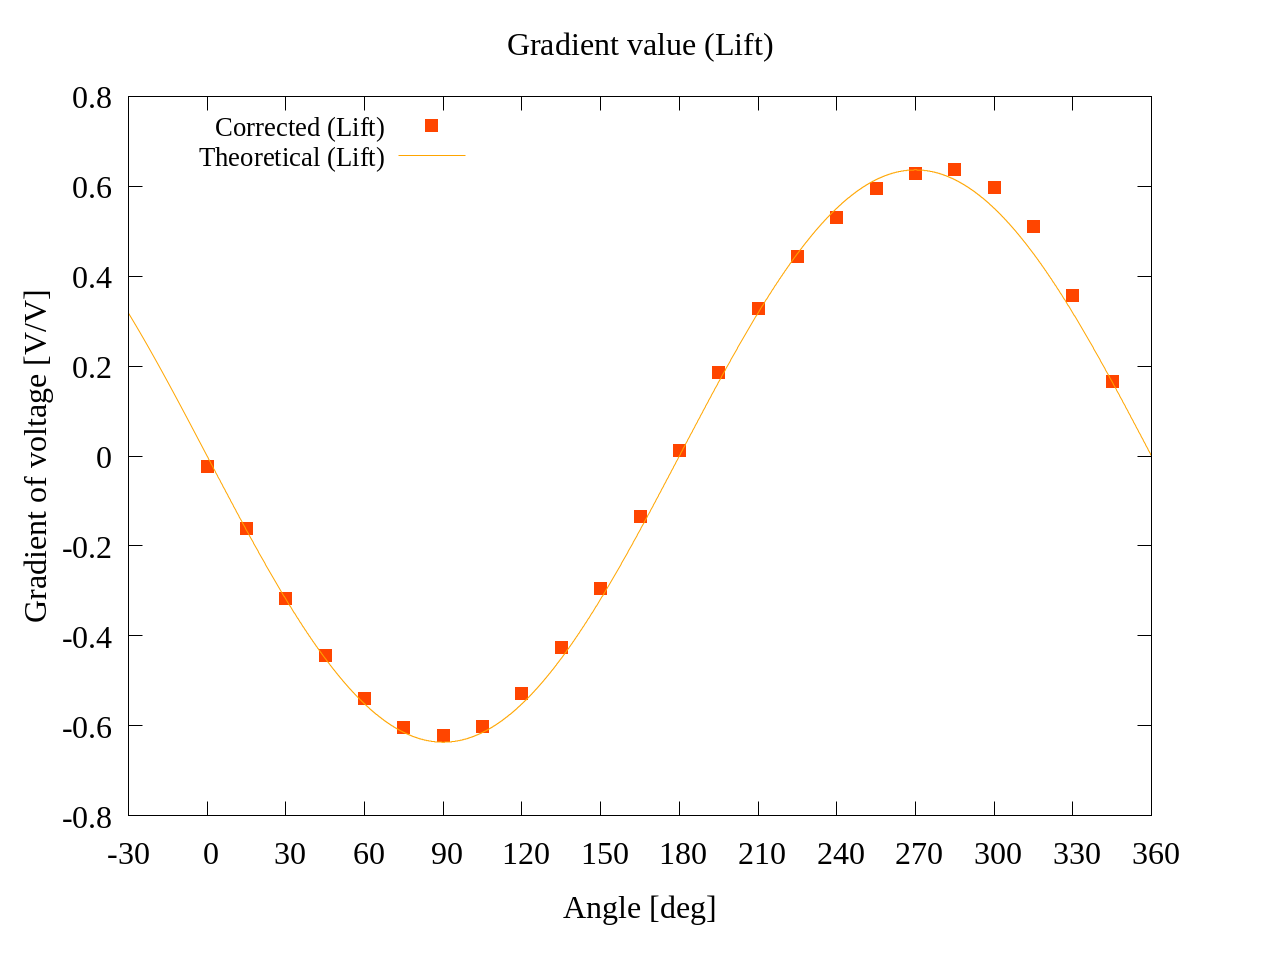
\includegraphics[width=86mm]{../graphes/1-ex/21/21-2_corrected_lift.png}
        \caption{Summary of lift's gradient voltage (corrected)}
    \end{center}
\end{figure}

\newpage

\begin{itemize}
    \item [$\blacksquare$] \textgt{正味出力電圧}
\end{itemize}

\begin{figure}[htbp]
    \footnotesize
    \begin{center}
        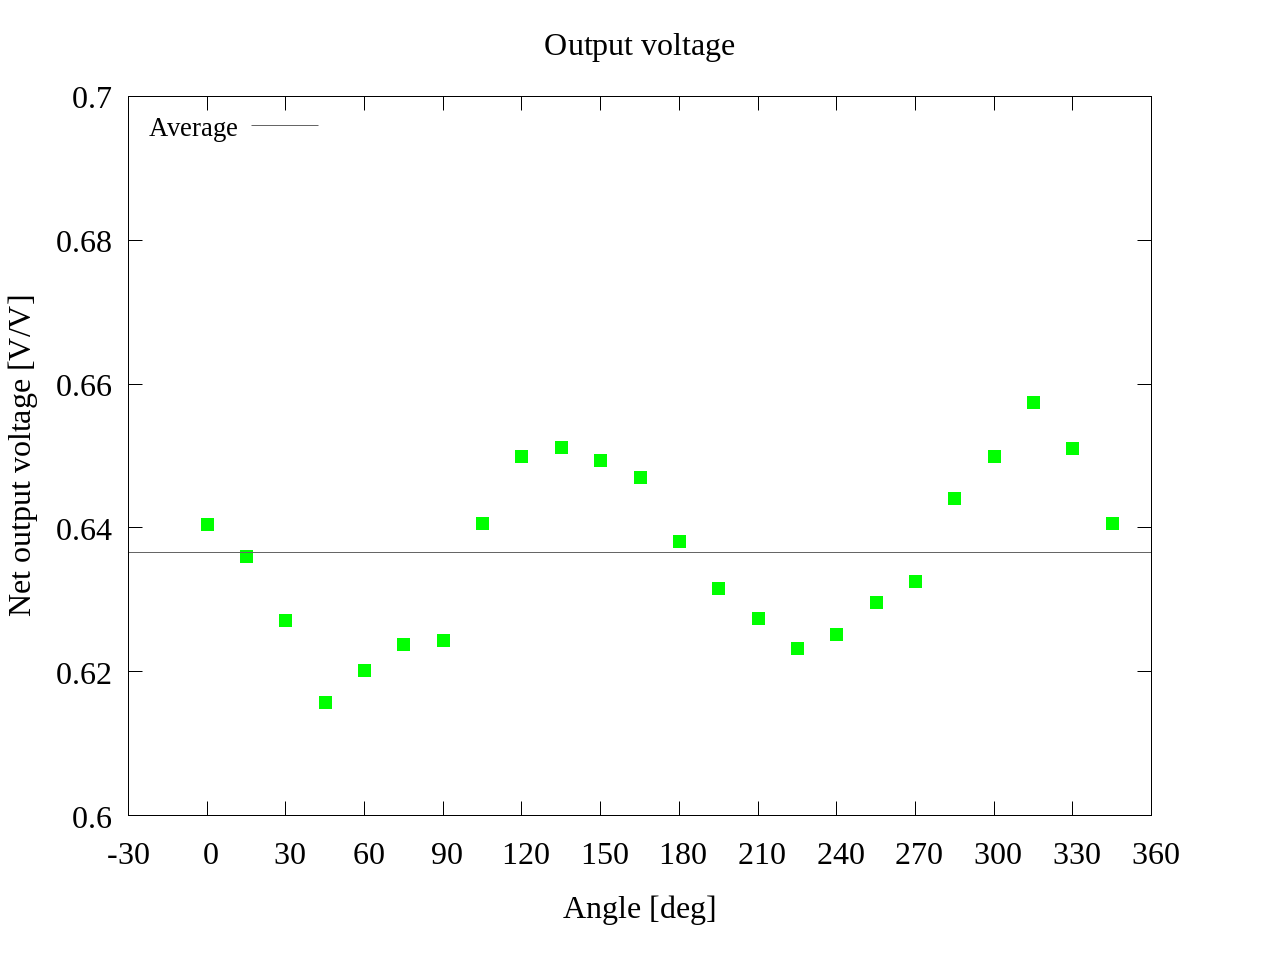
\includegraphics[width=86mm]{../graphes/1-ex/09/09_summary-outputvoltage-net.png}
        \caption{Summary of net voltage (Corrected)}
    \end{center}
\end{figure}

\begin{table}[htbp]
    \scalefont{0.9}
    \begin{center}
        \caption{Result summary}
        \begin{tabular}{|p{20mm}|p{20mm}|p{20mm}|p{20mm}|}
            \hline
            \multicolumn{1}{|c|}{\textgt{Angle [deg]}} & \multicolumn{1}{|c|}{\textgt{$A_d'$ [V/V]}} & \multicolumn{1}{|c|}{\textgt{$A_l'$ [V/V]}} & \multicolumn{1}{|c|}{\textgt{$A_{net}$ [V/V]}} \\ \hline
            \multicolumn{1}{|c|}{0}                    & \multicolumn{1}{|r|}{-0.640}                & \multicolumn{1}{|r|}{\textgt{-0.022}}       & \multicolumn{1}{|r|}{\textgt{0.640}}           \\ \hline
            \multicolumn{1}{|c|}{15}                   & \multicolumn{1}{|r|}{-0.615}                & \multicolumn{1}{|r|}{\textgt{-0.161}}       & \multicolumn{1}{|r|}{\textgt{0.636}}           \\ \hline
            \multicolumn{1}{|c|}{30}                   & \multicolumn{1}{|r|}{-0.541}                & \multicolumn{1}{|r|}{\textgt{-0.317}}       & \multicolumn{1}{|r|}{\textgt{0.627}}           \\ \hline
            \multicolumn{1}{|c|}{45}                   & \multicolumn{1}{|r|}{-0.428}                & \multicolumn{1}{|r|}{\textgt{-0.443}}       & \multicolumn{1}{|r|}{\textgt{0.616}}           \\ \hline
            \multicolumn{1}{|c|}{60}                   & \multicolumn{1}{|r|}{-0.307}                & \multicolumn{1}{|r|}{\textgt{-0.539}}       & \multicolumn{1}{|r|}{\textgt{0.620}}           \\ \hline
            \multicolumn{1}{|c|}{75}                   & \multicolumn{1}{|r|}{-0.154}                & \multicolumn{1}{|r|}{\textgt{-0.604}}       & \multicolumn{1}{|r|}{\textgt{0.624}}           \\ \hline
            \multicolumn{1}{|c|}{90}                   & \multicolumn{1}{|r|}{0.045}                 & \multicolumn{1}{|r|}{\textgt{-0.623}}       & \multicolumn{1}{|r|}{\textgt{0.624}}           \\ \hline
            \multicolumn{1}{|c|}{105}                  & \multicolumn{1}{|r|}{0.219}                 & \multicolumn{1}{|r|}{\textgt{-0.602}}       & \multicolumn{1}{|r|}{\textgt{0.641}}           \\ \hline
            \multicolumn{1}{|c|}{120}                  & \multicolumn{1}{|r|}{0.378}                 & \multicolumn{1}{|r|}{\textgt{-0.529}}       & \multicolumn{1}{|r|}{\textgt{0.650}}           \\ \hline
            \multicolumn{1}{|c|}{135}                  & \multicolumn{1}{|r|}{0.493}                 & \multicolumn{1}{|r|}{\textgt{-0.425}}       & \multicolumn{1}{|r|}{\textgt{0.651}}           \\ \hline
            \multicolumn{1}{|c|}{150}                  & \multicolumn{1}{|r|}{0.578}                 & \multicolumn{1}{|r|}{\textgt{-0.295}}       & \multicolumn{1}{|r|}{\textgt{0.649}}           \\ \hline
            \multicolumn{1}{|c|}{165}                  & \multicolumn{1}{|r|}{0.633}                 & \multicolumn{1}{|r|}{\textgt{-0.134}}       & \multicolumn{1}{|r|}{\textgt{0.647}}           \\ \hline
            \multicolumn{1}{|c|}{180}                  & \multicolumn{1}{|r|}{0.638}                 & \multicolumn{1}{|r|}{\textgt{0.013}}        & \multicolumn{1}{|r|}{\textgt{0.638}}           \\ \hline
            \multicolumn{1}{|c|}{195}                  & \multicolumn{1}{|r|}{0.604}                 & \multicolumn{1}{|r|}{\textgt{0.186}}        & \multicolumn{1}{|r|}{\textgt{0.632}}           \\ \hline
            \multicolumn{1}{|c|}{210}                  & \multicolumn{1}{|r|}{0.534}                 & \multicolumn{1}{|r|}{\textgt{0.329}}        & \multicolumn{1}{|r|}{\textgt{0.627}}           \\ \hline
            \multicolumn{1}{|c|}{225}                  & \multicolumn{1}{|r|}{0.436}                 & \multicolumn{1}{|r|}{\textgt{0.445}}        & \multicolumn{1}{|r|}{\textgt{0.623}}           \\ \hline
            \multicolumn{1}{|c|}{240}                  & \multicolumn{1}{|r|}{0.331}                 & \multicolumn{1}{|r|}{\textgt{0.530}}        & \multicolumn{1}{|r|}{\textgt{0.625}}           \\ \hline
            \multicolumn{1}{|c|}{255}                  & \multicolumn{1}{|r|}{0.205}                 & \multicolumn{1}{|r|}{\textgt{0.595}}        & \multicolumn{1}{|r|}{\textgt{0.630}}           \\ \hline
            \multicolumn{1}{|c|}{270}                  & \multicolumn{1}{|r|}{0.065}                 & \multicolumn{1}{|r|}{\textgt{0.629}}        & \multicolumn{1}{|r|}{\textgt{0.633}}           \\ \hline
            \multicolumn{1}{|c|}{285}                  & \multicolumn{1}{|r|}{-0.096}                & \multicolumn{1}{|r|}{\textgt{0.637}}        & \multicolumn{1}{|r|}{\textgt{0.644}}           \\ \hline
            \multicolumn{1}{|c|}{300}                  & \multicolumn{1}{|r|}{-0.258}                & \multicolumn{1}{|r|}{\textgt{0.596}}        & \multicolumn{1}{|r|}{\textgt{0.650}}           \\ \hline
            \multicolumn{1}{|c|}{315}                  & \multicolumn{1}{|r|}{-0.413}                & \multicolumn{1}{|r|}{\textgt{0.512}}        & \multicolumn{1}{|r|}{\textgt{0.657}}           \\ \hline
            \multicolumn{1}{|c|}{330}                  & \multicolumn{1}{|r|}{-0.545}                & \multicolumn{1}{|r|}{\textgt{0.356}}        & \multicolumn{1}{|r|}{\textgt{0.651}}           \\ \hline
            \multicolumn{1}{|c|}{345}                  & \multicolumn{1}{|r|}{-0.619}                & \multicolumn{1}{|r|}{\textgt{0.166}}        & \multicolumn{1}{|r|}{\textgt{0.641}}           \\ \hline \hline
            \multicolumn{1}{|c|}{Average}              & \multicolumn{1}{|r|}{0.023}                 & \multicolumn{1}{|r|}{\textgt{0.013}}        & \multicolumn{1}{|r|}{\textgt{0.637}}           \\ \hline
        \end{tabular}
    \end{center}
\end{table}

\newpage

\section{校正装置と実験装置の軸のオフセット}

以前の補正理論では,実験装置と校正装置の軸の回転によるズレに着目し補正を行った.
しかし,そこから算出された正味出力電圧は一定値を示すことはなく,周期的な振動を示すような結果(Fig.4)を示した.\par
ここで,校正装置と実験装置の軸にオフセット(Fig.5)があることがその要因の一つと考えられる.
このオフセットについては,人為的な装置の設置過程では無視することが不可能な誤差である.
したがって,オフセットを考慮したテストデータを作成しその結果を見ることで
正味出力電圧における周期的な振動の原因・影響の大きさを調べる.

\begin{figure}[htbp]
    \footnotesize
    \begin{center}
        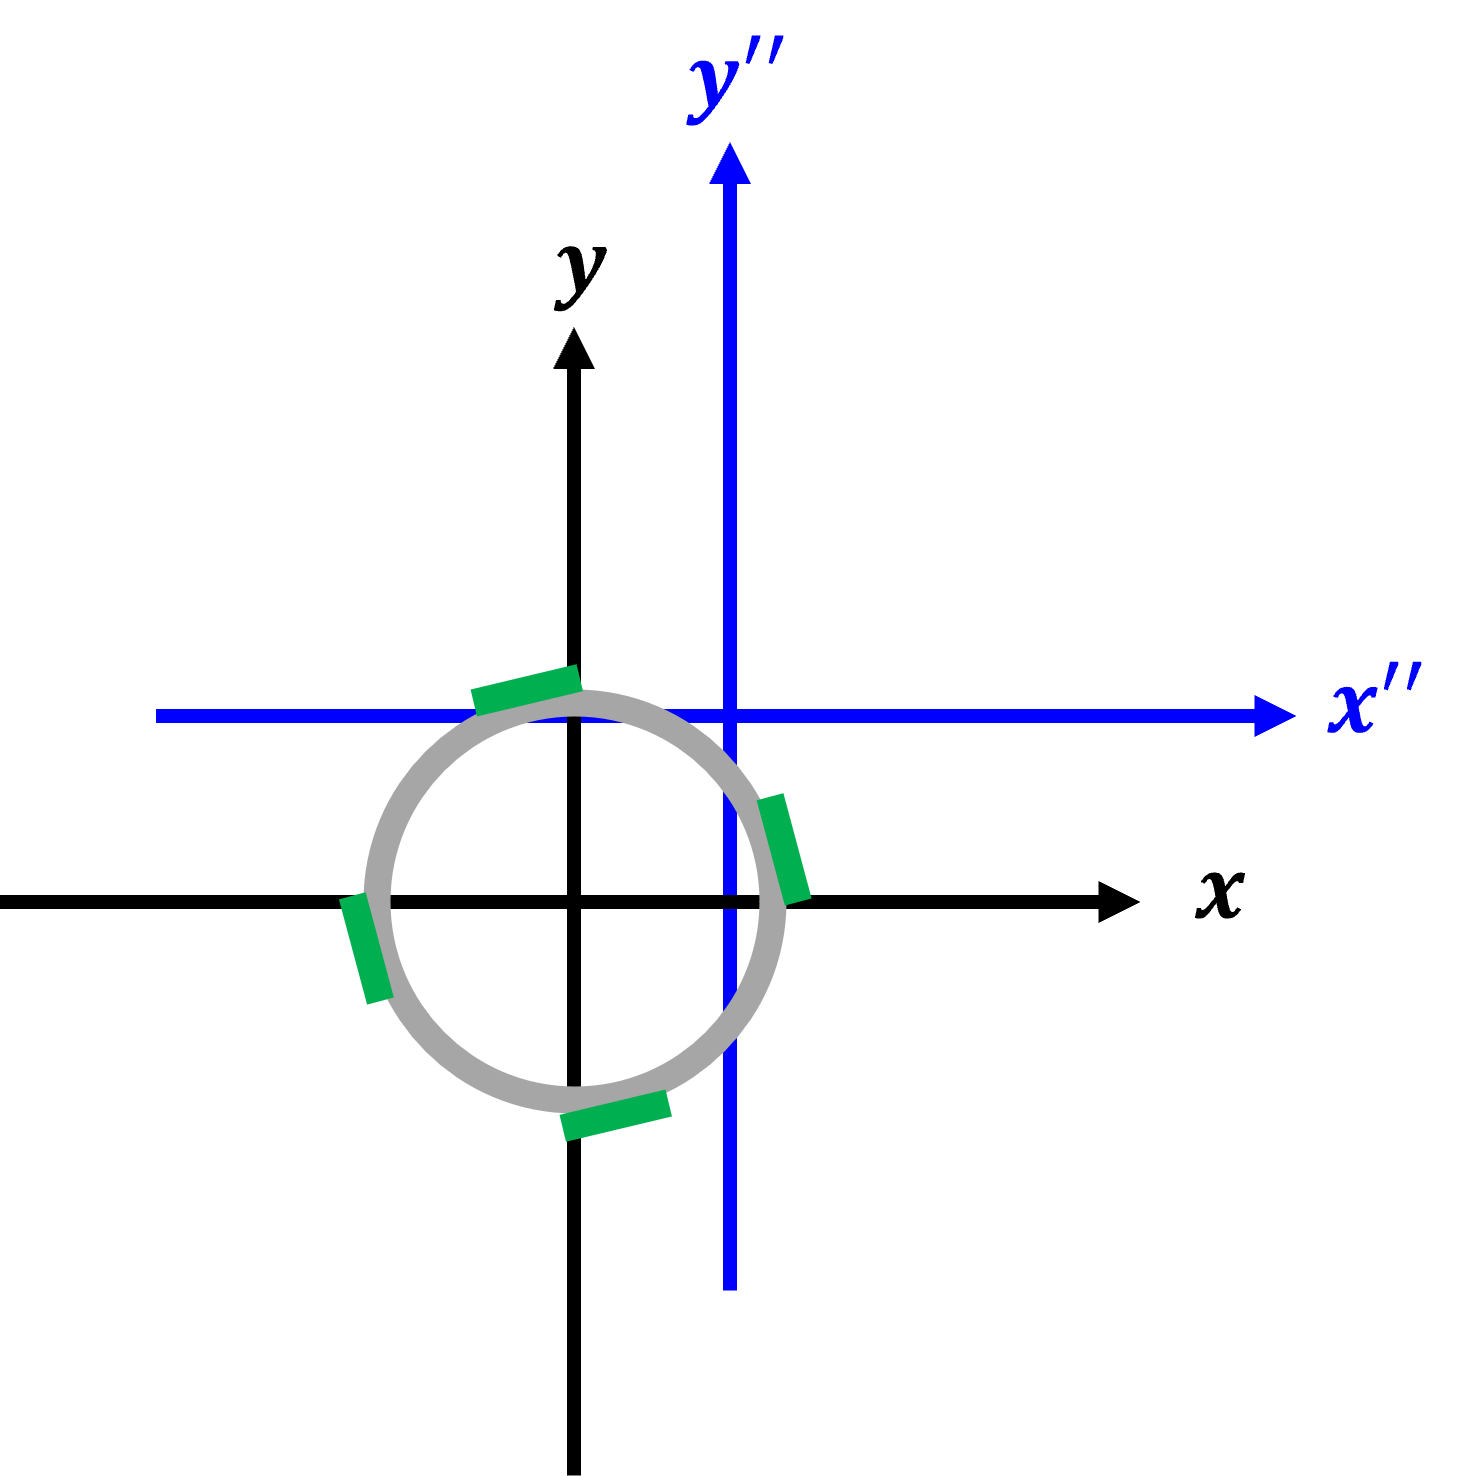
\includegraphics[width=70mm]{../images/image_5.png}
        \caption{}
    \end{center}
\end{figure}

\newpage

\subsection{オフセットによる出力電圧への影響}

はじめに,正規座標系$x-y$より,$\Delta x$,$\Delta y$だけ
移動した座標系$x''-y''$を校正装置における座標系とする.
ここで,供試体表面に任意の角度$\theta$から作用力$F$を加える.
このとき,作用力$F$は,$\Delta x$,$\Delta y$のオフセットを持つため,
正規座標系における中心$o$を通ることはない.

\begin{figure}[htbp]
    \footnotesize
    \begin{center}
        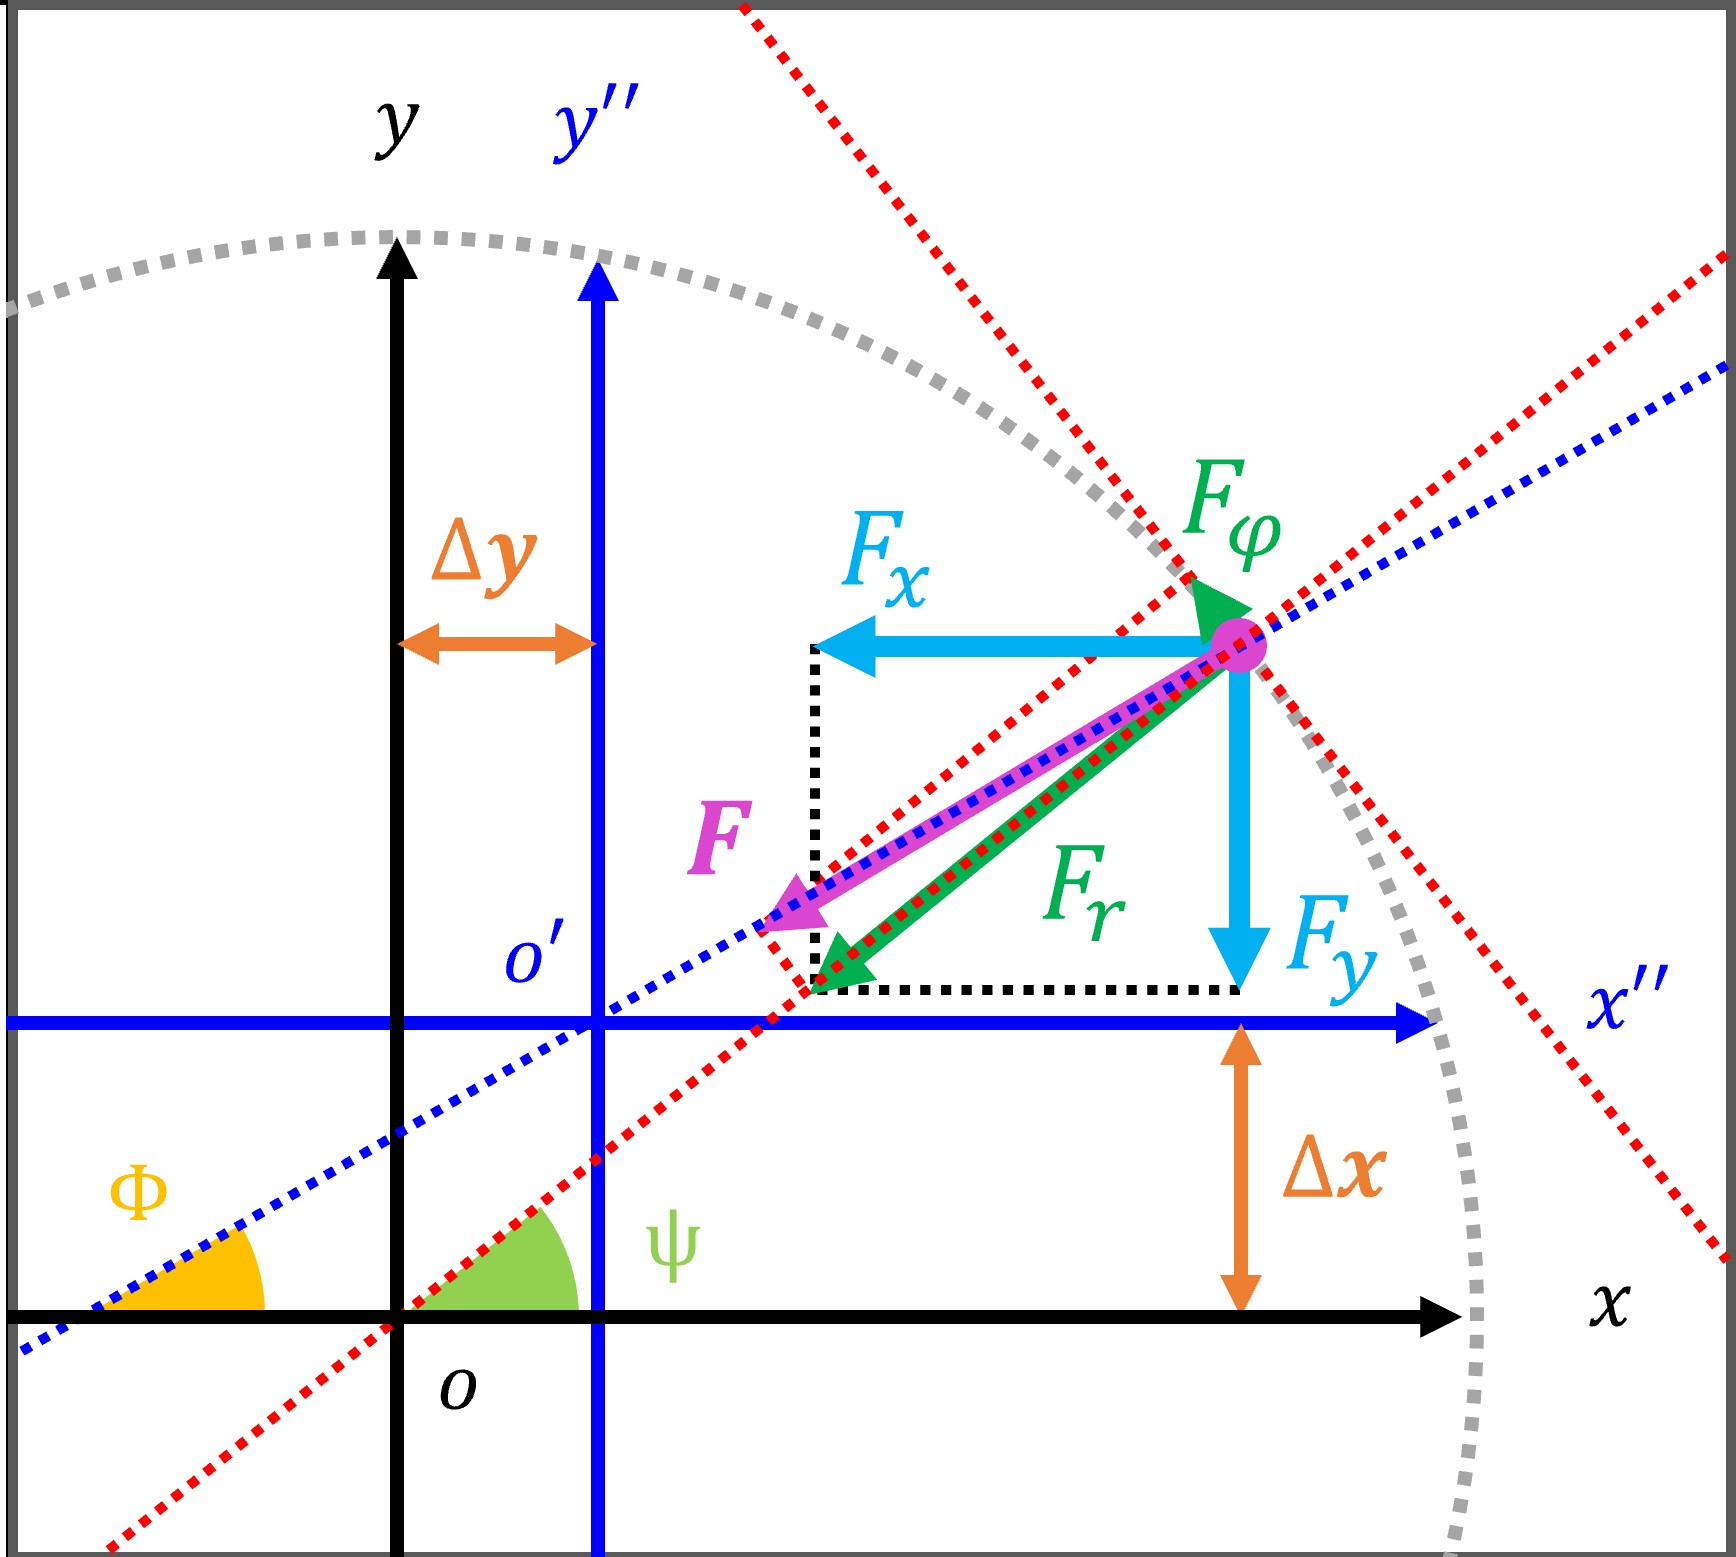
\includegraphics[width=80mm]{../images/image_6.png}
        \caption{}
    \end{center}
\end{figure}

\subsection{角度$\psi$の算出}

\subsection{作用力の$F_r$,$F_\psi$への分解とトルク$T$の影響}

供試体に加わる作用力$F$は供試体表面の接線方向の力$F_\varphi$,
またその法線方向の力$F_r$に分けて考えることができる.
算出した$\psi$を用いると,それぞれ以下のように求められる.

\begin{itemize}
    \item [$\blacksquare$] \textgt{接戦方向の力$F_\varphi$,接戦と法線方向の力$F_r$の算出}
          \begin{eqnarray*}
              F_\varphi &=& F \sin \psi \\
              F_r &=& F \cos \psi
          \end{eqnarray*}
\end{itemize}

接戦方向成分$F_\varphi$について,供試体に対してトルク$T$として作用することとなる.

\begin{itemize}
    \item [$\blacksquare$] \textgt{供試体へ作用するトルク$T$}
          \begin{eqnarray*}
              T &=& F_\varphi \cdot r\\
              &=& F \sin \psi \cdot r
          \end{eqnarray*}
\end{itemize}

ここで,このトルク$T$について,
作用力測定装置に対する影響は十分に小さいと考えられることから無視できる.

\end{document}